\chapter{網際內容如何提升教學與研究應用}
\renewcommand{\baselinestretch}{10} %設定行距
%\section{前言}
\par
\renewcommand{\baselinestretch}{2} %設定行距
\twelve 從教學與研究歷程的重要性作為研究動機,希望不只提供學生在學習與研究流程能夠不只留下具體成果,也能有效呈現更細部的歷程資料,以作為學習與研究更有力的佐證資料。
\par

\renewcommand{\baselinestretch}{20} %設定行距
\section{費曼學習法}
\par
\renewcommand{\baselinestretch}{1} %設定行距
\twelve 研究顯示,人類的學習型態分為以下兩種,而當兩種行為同時進行時,能使學習成效大幅提升。
\begin{itemize}
	\item 主動學習
	\item 被動學習
\end{itemize}
\par
\renewcommand{\baselinestretch}{1} %設定行距
\twelve 何謂被動學習? 老師傳播知識,而學生進行吸收,或是透過網路及大眾媒體接收資訊,這些都是常見的被動學習,也是人類大部分獲得知識的渠道。
\par
\renewcommand{\baselinestretch}{1} %設定行距
\twelve 主動學習則是,學習者在接收到資訊後,主動並有意識的思考,在腦中形成一個自己理解方式或產生其他疑問,再去透過尋找資料,主動研究,或是與人討論甚至透過教學等行動進行的學習方式。
\\
\par

\renewcommand{\baselinestretch}{20} %設定行距
\subsection{從費曼學習法的角度觀看}
\par
\renewcommand{\baselinestretch}{1} %設定行距
\twelve 現今華人地區的教學方式,最大的特徵就是「填鴨式」教育。華人的教師認為,他們在課堂上不得不放慢他們習慣的教學進度,因為學生聽不懂也記不住,他們期待學生將聽到的知識記下來,然後就可以應用,可是當這種教育放在國外會發現,很多學生都做不到這一點,他們總是要問「為什麼?,例如:為什麼這條輔助線要劃在這裡,為什麼這道題要這麼算......中方老師的教法,在某種程度上,其實就是一種「填鴨式」,你不需要了解這算法背後的原理,你只需要能夠處理這種算法,學會它並且應用它。可是外國學生對此接受無能,他們沒這個習慣,要在短時間內被「填入」這麼多知識,於是課堂進度被拖慢了。
\par

\renewcommand{\baselinestretch}{20} %設定行距
\subsection{費曼學習法的研究成效}
\par
\renewcommand{\baselinestretch}{1} %設定行距
\twelve 會發現我們的學生會習慣於「接受填鴨」這種僵化的方式去被動學習;反觀外國的學生,在他們的教學體制下,學生會敢於問「為甚麼?」,當他們問出這個問題,並且開始和老師同學討論時,學生就會處於主動學習的狀態了,這時他們的學習效果會大幅提升。\\
\par
\renewcommand{\baselinestretch}{1} %設定行距
\twelve 在生活環境中會有大量的資訊塞入我們的腦中,但是這些資訊屬於被動學習,實際吸收進去的只有不到30\%,而透過研究、紀錄、寫心得甚至教學的方式,與我們腦中的被動資訊相輔相成,可以使資訊吸收的效益增加到80\%~90\%。
\\
\par
\renewcommand{\baselinestretch}{1} %設定行距
\twelve 如(圖\ref{fig.學習金字塔})
\begin{enumerate}
	\item 講課: 授課只是純粹在學生面前說話,不涉及學生的參與,學生只能牢記當中5\% 的知識。
	\item 閱讀: 授課方式增加一個簡報或是參考資料,讓同學邊看邊閱讀,就會稍稍提高到10\%。
	\item 視聽: 授課時播放相關知識的影片,學生的知識牢記率,就會提升到20\%。
	\item 示範: 很多科學科為什麼會特別喜歡做實驗,因為示範比純粹說話好一點,學生的知識牢記率可以提升到30\%。
	\item 小組討論: 當學生直接參與整個學習過程,知識牢記率會大大提升。例如,小組活動,因為這樣就能夠將知識內化成自身的想法,然後再表達出來,這麼知識牢記率就能提升到50\%。
	\item 實踐: 實際動手比看著老師示範好,很多時候科學實驗是老師先做,然後學生再做實際動手,這樣知識牢記率就能提升到80\%。
	\item 教其他人: 最好的知識牢記方法是教其他人,原因是你內化再表達的時候,你會透過不斷教人而增強了對知識的記憶,而達到真正了解、完全吸收資訊。
\end{enumerate}
\par
\renewcommand{\baselinestretch}{1.7} %設定行距
\begin{figure}[hbt!]
\begin{center}
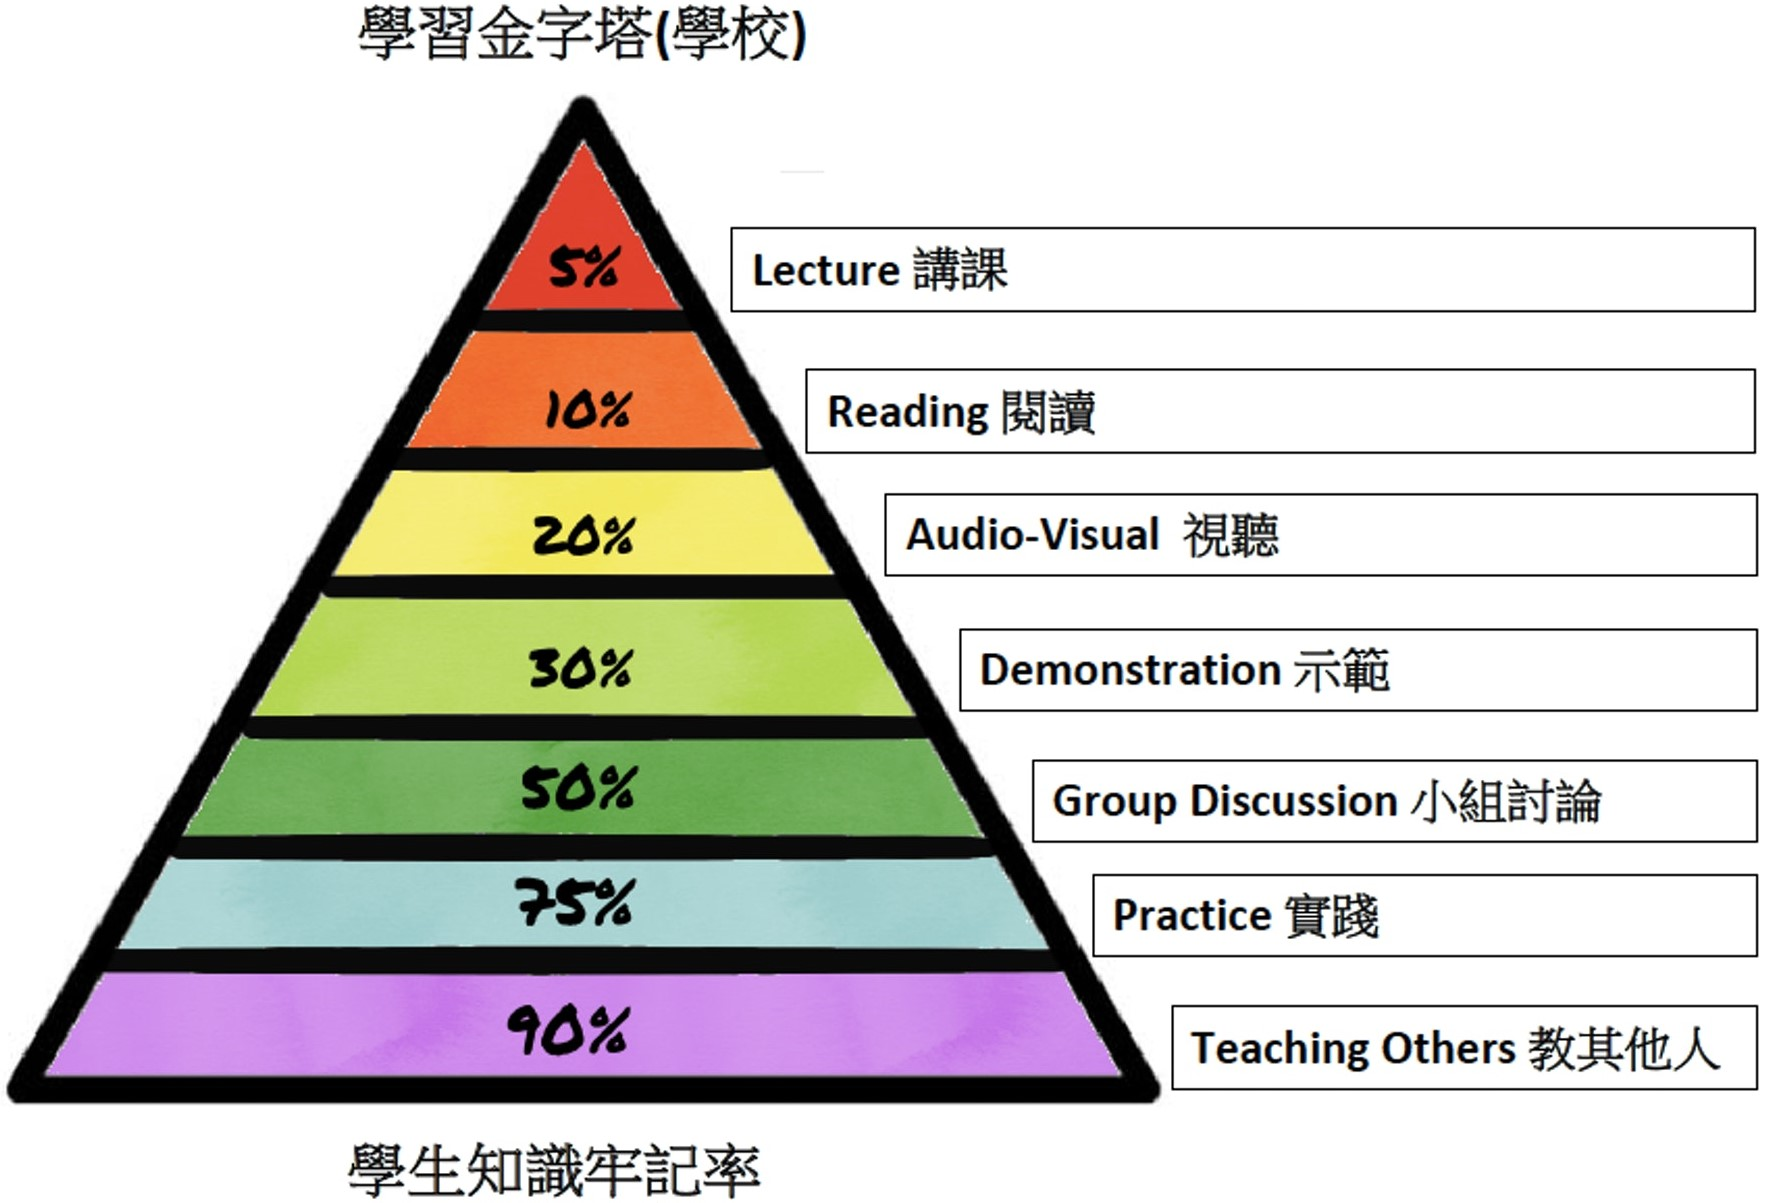
\includegraphics[width=4in]{21}
\caption{\large 學習金字塔}\label{fig.學習金字塔}
\end{center}
\end{figure}
\par

\renewcommand{\baselinestretch}{20} %設定行距
\section{數位化學習環境}
\par
\renewcommand{\baselinestretch}{1} %設定行距
\twelve 於是在數位化的社會下,開始有許多人利用網際內容資源,提供一個數位化學習環境,提升教學品質。\\
\par
\renewcommand{\baselinestretch}{1} %設定行距
\twelve 相比於一般學校裡的教學環境,數位化的網路教學系統可以更容易地設計出讓「使用者主動學習」的教學環境,比如架立討論平台,建立個人專案紀錄歷程檔案......。
\par

\renewcommand{\baselinestretch}{20} %設定行距
\subsection{如何設計出教學環境}
\par
\renewcommand{\baselinestretch}{1} %設定行距
\twelve 首先,我們可以透過費曼學習法,區分主動與被動學習,並分析出教學中,適合引導使用者行主動學習的要素,如以下的方式。
\begin{enumerate}
	\item 課程目標
	\begin{itemize}
		\item 為什麼要開這門課?
		\item 開這門課的目的是什麼?
		\item 希望達成什麼樣的目標?
		\item 希望解決什麼樣的問題?
		\item 達成這樣的目標對於個人、社會、世界會發生什麼樣的影響?
	\end{itemize}
	\item 理論基礎
	\begin{itemize}
		\item 為達成前述的目標,應該要如何結構一門課?
		\item 什麼樣的理論基礎及知識觀點可以支撐起這個架構?
	\end{itemize}
	\item 教學題材
	\begin{itemize}
		\item 選用什麼題材可以反應真實世界概況?
		\item 什麼實例可以串接學生及生活世界之間的距離?
		\item 什麼內容可以與時俱進並體現時代的脈動?
	\end{itemize}
「教學」中值得「研究」的元素
	\item 教學方法
	\begin{itemize}
		\item 設計何種教法可以合適地表達教材的意義?
		\item 規劃什麼樣的活動可以激發學生的動機,並且深化學習的意義?
	\end{itemize}
	\item 學生學習
	\begin{itemize}
		\item 學生如何建構對於知識的理解?
		\item 如何形成相關的態度?
		\item 學生學習及認知的過程為何?
	\end{itemize}
	\item 成果評量
	\begin{itemize}
		\item 經過教學之後,整體課程的效果如何?
		\item 如何明確地評量?
	\end{itemize}
\end{enumerate}
\par

\renewcommand{\baselinestretch}{20} %設定行距
\section{數位教育資源的實體功能}
\par
\renewcommand{\baselinestretch}{1} %設定行距
\twelve 分析完教學中,適合引導使用者主動學習的要素後,針對上述要點,我們可以規劃出一系列的教學網站結構。
\begin{enumerate}
	\item 測驗練習: 用軟體做題,不用等待老師長時間的批改,自己馬上就能知道自己的薄弱環節。
	\item 測驗詳解: 測驗完,針對自己不太會的,可以看到答題詳解,立即更正原本錯誤的觀念。
	\item 互動平台: 傳統的課堂,由於時間有限,無法廣泛聽取所有同學的觀點,再加上青春期的特點,即使有想法,有些孩子也總是羞於舉手回答,一定程度上影響了表達和共享,老師也很難知道學生的情況。課堂交流也不一定要面對面,讓學習跨越時空,一對一的課堂問答模式變成了面向全體的在線問答。多對多課堂模式,所有學生都可以看到「班級問答」區的問題,如此,交流不再是少部分同學的特權,每個人的機會都是均等的,這也在某種程度上重塑學生學習的信心。在線問答和交流,所有孩子都有機會及時整理自己的知識和想法,老師也能真正和孩子們互動起來。這種模式下的學習,打破了課堂時間和空間位置的束縛,增大信息流量,實現全班同學的思維互動。同時,也發揮了部分學有餘力的同學的資源優勢,最終提高了全體學生的學習積極性和學習績效。
	\item 個人紀錄: 查看已發觀點並進行適當地調整,最終將自己的觀點整理輸出。
	\item 背景後台: 針對不同的使用者,開放不同的權限,老師可以上傳了海量的學習資源,一鍵將不同難度的視頻推送給不同層次的學生;利用它進行課堂學習,同時也能給程度不一致的學生設置不同的課後習題,並且觀察到後台大數據,瞬間分析出每一個學生的作業正確率和做題速度等,每個學生解題答案老師一清二楚。
\end{enumerate}
\par
\renewcommand{\baselinestretch}{1} %設定行距
\twelve 將教師從知識的搬運工變成課堂教學活動的設計者、組織者、指導者與參與者;把學生從知識的背誦者、接受者變為知識的實踐者、探索者和創造者,自動學習,學會分享交流,並在討論中觸發創新,實現自主化、個性化的學習。
\par


\renewcommand{\baselinestretch}{20} %設定行距
\section{運用網際網路提升研究效益}
\par
\renewcommand{\baselinestretch}{1} %設定行距
\twelve 俗話說「事半功倍」,指的是不論做什麼事情,只要方法對了,必定可以用最少的力氣與成本完成最多的工作,進而提升工作上的效率;而做研究也是一樣,要有一套正確的方法,就可以達到「事半功倍」的效果。或許有人會質疑說,做研究是非常困難的一件事,需要有非常廣博的知識、堅實的學理根基才行,但是,只要你掌握住研究的要領以及方法且多善用數據分析,也仍能可以有效率地推展完成,進而從容改進,並達到超乎預期的良好品質要求。
\\
\par
\renewcommand{\baselinestretch}{1} %設定行距
\twelve 而研究的面向包含三個:一是教學策略(pedagogy,包含教具研發、教材開發、教學方式創新、學習策略、課程與教學創新,如MOOCS等);二是教學空間(space,學習者中心的教室規劃、座位安排,如高互動教室等);三為教學科技(technology,行動學習、3D科技、VR與AR等),三個面向彼此輔助、活化、提升。
\\
\par
\renewcommand{\baselinestretch}{1} %設定行距
\twelve 以往只能透過圖書館、人脈網絡尋找的資料,現在已能透過網路以較低的時間成本、勞力與財務成本獲得,對個人來說,學習變成即時、隨時隨地、與不得不為的事情,也使學習這件事不再有城鄉差距,讓學習這件事情變得更有意義,而在資訊爆炸的時代,如何從龐雜且倍速成長的資料中,擷取出具有意義和應用價值的內容尤為重要,大數據(Big Data)結合AI人工智慧的數位應用,是有效提升工作效率及產值的關鍵。
\\
\par
\renewcommand{\baselinestretch}{1} %設定行距
\twelve 對於學生而言,學術資訊獲取的管道非常多元,除了教科書、期刊文獻、網路、教育單位或是學術論壇,進而學習與吸收獲取的知識,而網際網路有別於傳統的模式,更不一樣的是學習模式的影響及轉變,也形成一種能由資訊科技來促進學習效能的模式;而達到探究知識的方法和歷程與自我省思,這些資料可進一步用來評量且取代單純以測驗或研究報告來代表學習者的學習成績。
\\
\par
\renewcommand{\baselinestretch}{1} %設定行距
\twelve 在網路的教學環境下,數位式的教材扮演重要的角色,因為在「電子教室」的教學環境下,學習活動並不只在課堂上進行。這時網路上的課程輔助教材,對學習活動形成很大的影響。目前網路上的教材設計多利用「全球資訊網」(簡稱WWW)上資源開發而成,期望利用多媒體呈現的能力,來豐富教學內容與增加學習者的了解。然而如何才能有效的發揮教材功能?教師在教材的設計上有那些要項?根據文獻探討得知,Mengel[Mengel 1996]指出目前WWW上的教材,其主要缺失為;「不易學習」、「不具可攜性」、「欠缺知識呈現的結構化」、「不易更新與維護」、以及「超鏈結(Hyperlink)方式不恰當」等,並且提出「超本文(Hypertext)課程設計的方法論」。
\\
\par
\renewcommand{\baselinestretch}{1} %設定行距
\twelve 總結以上資訊可得知「科技的進步是以滿足人類的需要為主」,它代表資訊科技在技術面與應用面的發展指標,應不斷思考其對人們需求所產生的衝擊。網路科技的進步,形成對教育環境與型式的重大改變。
\par
\renewcommand{\baselinestretch}{1} %設定行距
\twelve 網際網路對於教學及研究上的影響與幫助,除了可以藉由學習心得 與作品之收錄、展示,可以讓學習者之間相互觀摩及學習,而透過自評,學習者可以自我檢視,發現問題,進而自我改善;也因為資訊數量過多,個人的資訊素養能力,比起以往時代,是一個更為重要的課題。一方面能幫助我們更有效率的處理日常生活資訊。但也有可能,讓我們陷入過度僵化的模式中,反而失去了真正對資訊品質覺察的判斷力,所以應該要能保持懷疑的態度與習慣,進而去分析與評估資訊的正確與錯誤,並且做出判斷與方法,才是達到學術研究的目的。
\par



\renewcommand{\baselinestretch}{20} %設定行距
\section{國內外的教學實踐與研究}
\par
\renewcommand{\baselinestretch}{1} %設定行距
\twelve 「Practice」一詞有「教學實務」與「教學實踐」兩種說法,不過本次的重點都還是放在「研究」(Research)。教育部規定,教學實務的升等途徑大致包含以下要素:將學生的學習成效從質與量的層面來分析其教學是否能提升學生的學習成效;在課程、教材、教法、教具、科技媒體應用與評量等有創新、改進或延伸應用的具體研發成果;或在校內外推廣具有重要貢獻者,皆可以「技術報告」送審,不過仍須以兩年內的公開發表為主,因此修訂擬改為「教學實踐研究升等」。
\par

\renewcommand{\baselinestretch}{1} %設定行距
\twelve  當教育部推動「補助大專院校教學實踐研究計畫」,有助於推動高等教育的課堂教學實踐研究,也樹立教學學術研究新的里程碑,促使「教學實踐研究與升等」能受到學術肯定與支持,同時也能提升教學在大學裡的地位。
\par

\renewcommand{\baselinestretch}{20} %設定行距
\subsection{基礎研究計畫之效益}
\par
\renewcommand{\baselinestretch}{1} %設定行距
\twelve 現在越來越多國家會去針對基礎研究計畫進行效益的邏輯編排,其中也會特別注重研究流程,並且進行中、長期的追蹤管理。
\par
\renewcommand{\baselinestretch}{20} %設定行距
\subsection{MSIT基礎研究邏輯架構}
\par
\renewcommand{\baselinestretch}{1} %設定行距
\twelve 南韓科學與資通訊部(Ministry of Science and ICT, MSIT)所制訂基礎研究計畫之邏輯架構,不僅有利於各部會進行基礎研究計畫時了解不同時間下所需關注之潛在績效指標,促使計畫管理者發展相關測量方法,並透過資料庫平台彙整績效資料以利計畫之績效監測。
\\
\par
\renewcommand{\baselinestretch}{1} %設定行距
\twelve 可以發現邏輯架構可回饋後續基礎研究計畫效益評估之決策依據,例如審查專家進行每項評估問題時,可綜整這些績效指標之表現進行證據導向之決策(Evidence based Decision-Making)。
\par
\begin{figure}[hbt!]
\begin{center}
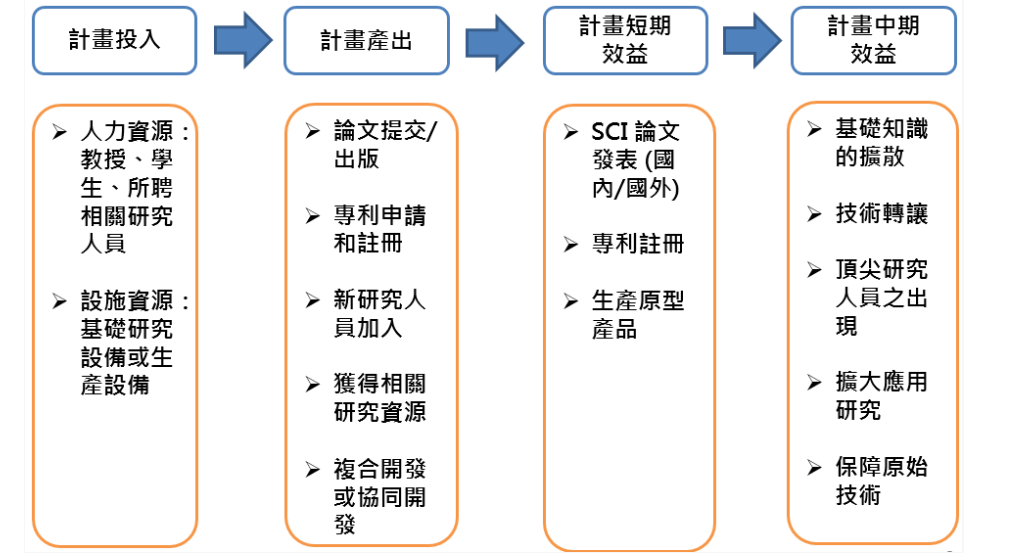
\includegraphics[width=5in]{33}
\caption{\large 研究計畫之邏輯架構}\label{fig.研究計畫之邏輯架構}
\end{center}
\end{figure}
\par

\renewcommand{\baselinestretch}{20} %設定行距
\subsection{JSPS基礎研究規劃}
\par
\renewcommand{\baselinestretch}{1} %設定行距
\twelve  日本學術振興會(Japan Society for The Promotion Science, JSPS) 基礎研究計畫結束時之評估,除了可綜觀了解整體執行之情況,亦能從評估過程中獲得改善未來基礎研究內容規劃之寶貴意見。
\par
\begin{figure}[hbt!]
\begin{center}
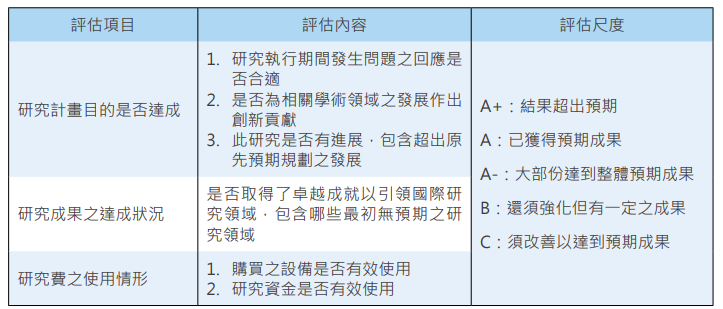
\includegraphics[width=5in]{34}
\caption{\large JSPS規劃之評估項目}\label{fig.JSPS規劃之評估項目}
\end{center}
\end{figure}
\par
\renewcommand{\baselinestretch}{20} %設定行距
\subsection{ERC補助計畫}
\par
\renewcommand{\baselinestretch}{1} %設定行距
\twelve 歐洲研究委員會(European Research Council, ERC)為補助歐洲境內進行基礎研究之重要科研機關,支持研究人員進行提案或由下而上(Bottom-Up)之前沿研究(Frontier Research)。ERC在最新一次(2017年)對所補助計畫之事後效益評估架構便設立兩個部份(整體評估、分項獨立評估)之效益評估問題(ERC, 2018),表2呈現評估問題及相關所需之評估尺度。透過這些評估問題有利於審查人員能有系統性地評估計畫效益,進行交叉列聯表分析例如可了解「計畫整體評分等級愈高(如整體評量對科學有重大突破或進展),是否計畫之跨領域效應(Q5)、計畫對於經濟、社會,以及政策制定效益影響面向。
 \par
\renewcommand{\baselinestretch}{1} %設定行距
\twelve 此外,ERC亦透過此評量結果與先前年度之評估結果進行比較,以了解不同年度之整體評估結果是否比先前有較佳之科學貢獻,例如ERC於最新一次(2017年)之效益評估會與前兩次之整體評估結果(2015與2016年)進行科學貢獻之比較。
\par
\begin{figure}[hbt!]
\begin{center}
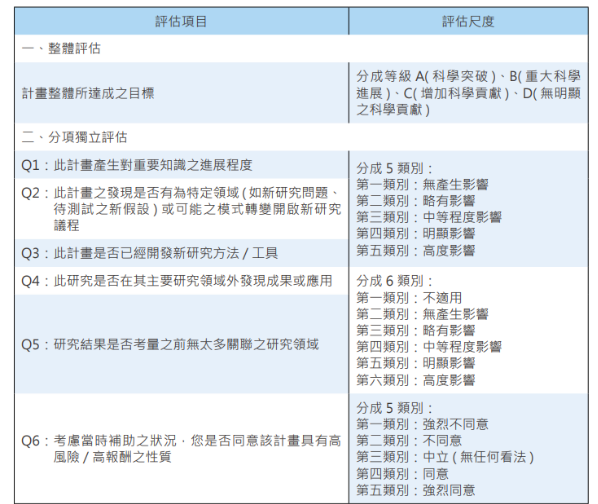
\includegraphics[width=5in]{35}
\caption{\large ERC規劃之評估項目}\label{fig.ERC規劃之評估項目}
\end{center}
\end{figure}
\par
\begin{figure}[hbt!]
\begin{center}
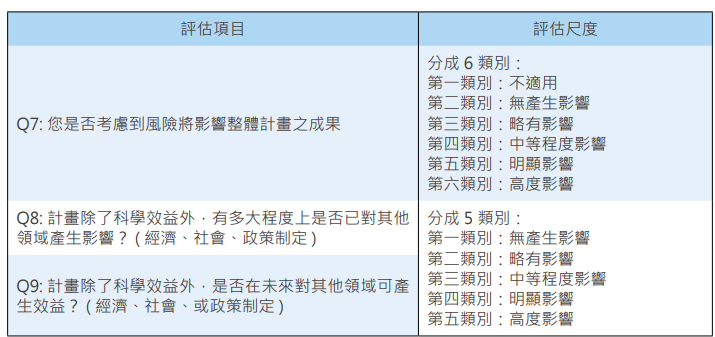
\includegraphics[width=5in]{36}
\caption{\large ERC規劃之評估項目}\label{fig.ERC規劃之評估項目}
\end{center}
\end{figure}
\par

\renewcommand{\baselinestretch}{20} %設定行距
\section{網際網路-遠距新趨勢}
\par
\renewcommand{\baselinestretch}{1} %設定行距
\twelve
\begin{enumerate}
	\item 電子郵件: 學生可利用電子郵件接收課程教材、作業分配、班級的相關資訊、並與教師、同學或不同年紀的學生相互溝通。教師也可另外設定一個課程討論群組(course listserv),所有的討論和問題都會寄到課程討論群組的電子郵件寄住信箱來,系統會自動將這些内容再寄給各組成員。
	\item 公告欄: 學生直接將自己的討論和間題張貼(post)在公告欄、公開討論區或新閒群組上,以相互溝通。使用者必須連到主機伺服器去閱覽這些文章。這樣可以有組纖的交談,因爲使用者可以選擇自己有興趣的主題進行閱讀和回應。
	\item 資料下載
學生可透過以下幾種方式獲取教學資料:利用檔案傳輸下載文件、教材或軟體;公告欄下載主題文章:全球資訊網下載所需的資料。這些資料下載之後:可在學生的電腦中閱讀或列印。這種方式最缺乏互動性,但卻是透過網際網路進行遠距教學或训練最常使用的方式。
	\item 互動式個別指導教材(Interaotive tutorial)
學生連線到網際網路上(通常是全球資訊網,並在線上取得個別指導教材。道些教材包括閱讀資料、連結到新的網站、回答問題或測驗等。有些個別指導教材允許學生依照自己的速度進行學習,每次連線進來都可繼續上次未完成的學習。
	\item 即時互動會議系統(Real-time Conference)
電子佈告欄和電子郵件在遠距學習的環境中屬於非同步學習。而「即時互動會議系統」則屬於同步學習,教師與學生同時在線上進行面對面的教學與討論。這是最接近傅統教室教學情境的一種方式,教師與學生或學生之間可即時的交談與間答。即時互動會議系統可採用多物件導向系統(Muti-user Object Oriented; MOOs),這是一個可以讓許多使用者同時進入的互動系統,例如網路聊天室 (Internet Relay Chat ; IRC) 便提供了許多即時學習和互動的機會。
	\item 全球資訊網: 以多媒體的方式(如文字、圖片。影像、動畫、聲音,等)提供各式各樣的資訊。大部份全球賌訊網的瀏覽器可以同時使用檔案找尋系統(Archie)、檔案傳輸、資料查詢服務系統、新閒論壇、電子郵件等資源。教師與學生可利用上述資源搜尋、列印、和下載資訊。全球資訊網不僅能夠整合網路的資源,還可讓使用者以建立網頁(Homepage)的方式,來成爲個人資訊提供者,而不單只是一個資訊使用者。道種整合運用資訊及讓使用者參與資訊建設的功能,使全球資訊網成為不可忽融的新教學媒體。
\end{enumerate}
\par

\renewcommand{\baselinestretch}{20} %設定行距
\section{運作方式}
\par
\renewcommand{\baselinestretch}{1} %設定行距
\twelve 利用Fossil SCM中的Forum(論壇)功能,學生或者其他使用者可以透過@gmail帳號登入,在論壇上進行互動,包含學校課程相關資訊、成果分享或其他使用者經歷分想等,也可以藉由@gm帳號在伺服器上建立一個自己的倉儲系統,可以利用分散式系統或其他功能建立自己的學習履歷、作業、作品等。
\\
\par
\begin{figure}[hbt!]
\begin{center}
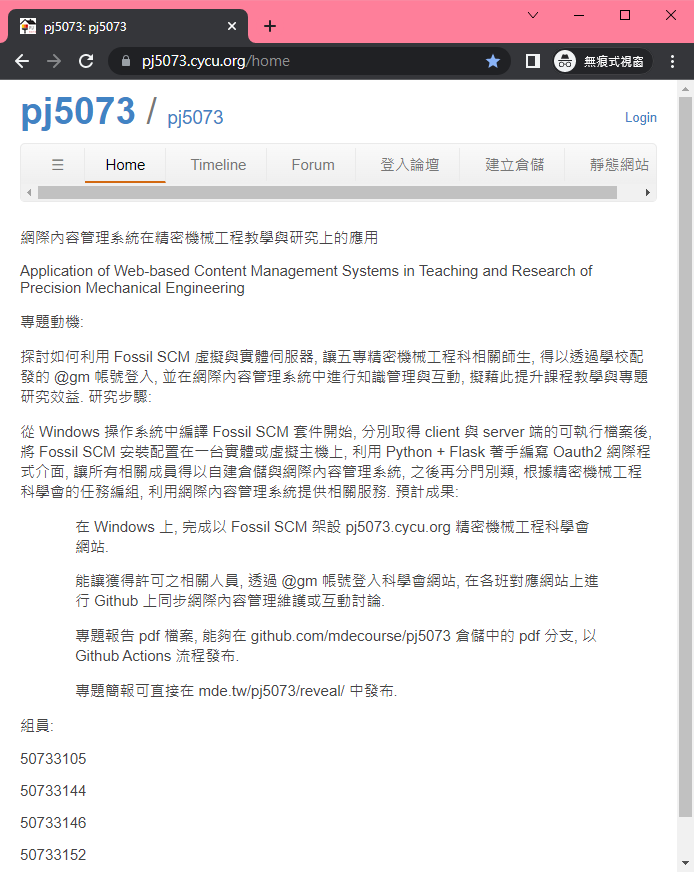
\includegraphics[width=4in]{22}
\caption{\large 網站}\label{fig.網站}
\end{center}
\end{figure}
\par
\twelve 論壇運作如(圖.\ref{fig.論壇})、(圖.\ref{fig.論壇資訊1})、(圖.\ref{fig.論壇資訊2})。
\\
\par
\begin{figure}[hbt!]
\begin{center}
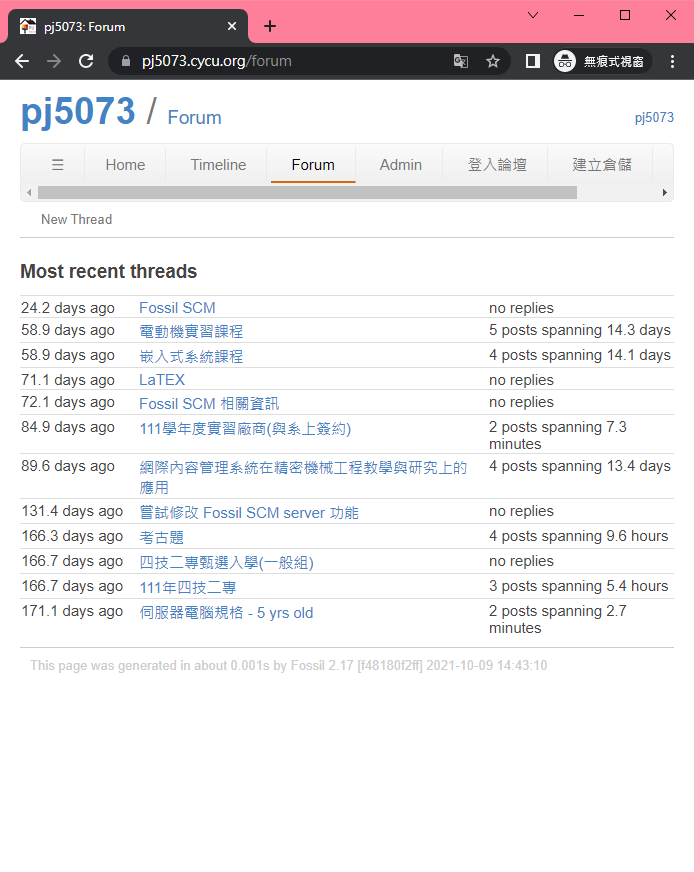
\includegraphics[width=5in]{23}
\caption{\large 論壇}\label{fig.論壇}
\end{center}
\end{figure}
\par
\begin{figure}[hbt!]
\begin{center}
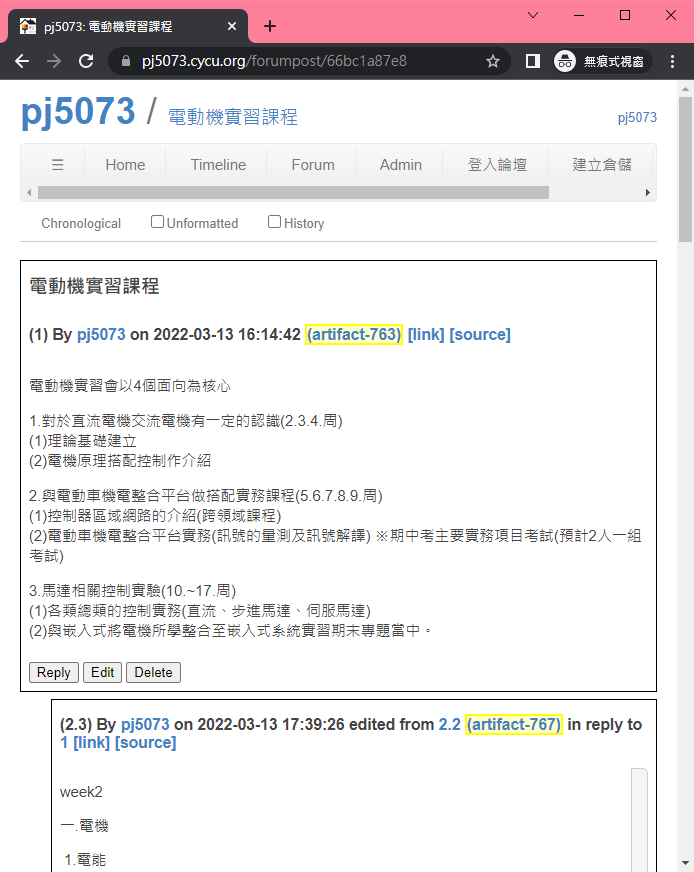
\includegraphics[width=5in]{24}
\caption{\large 論壇資訊1}\label{fig.論壇資訊1}
\end{center}
\end{figure}
\par
\begin{figure}[hbt!]
\begin{center}
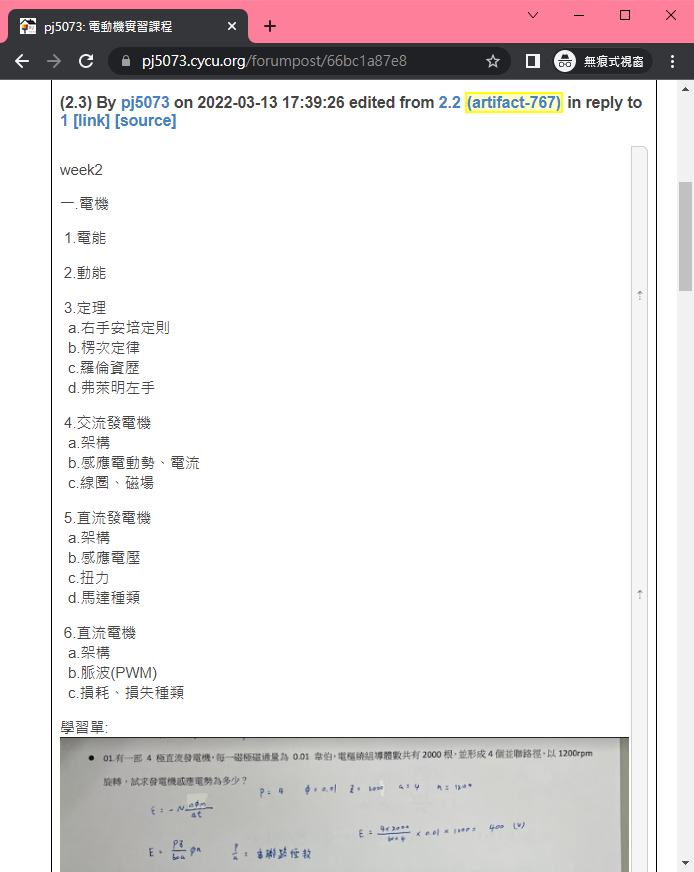
\includegraphics[width=5in]{25}
\caption{\large 論壇資訊2}\label{fig.論壇資訊2}
\end{center}
\end{figure}
\par
\twelve 分散式系統中最突出功能為版本控制,可以完全記錄整個歷程如(圖.\ref{fig.本版控制})。
\\
\par
\begin{figure}[hbt!]
\begin{center}
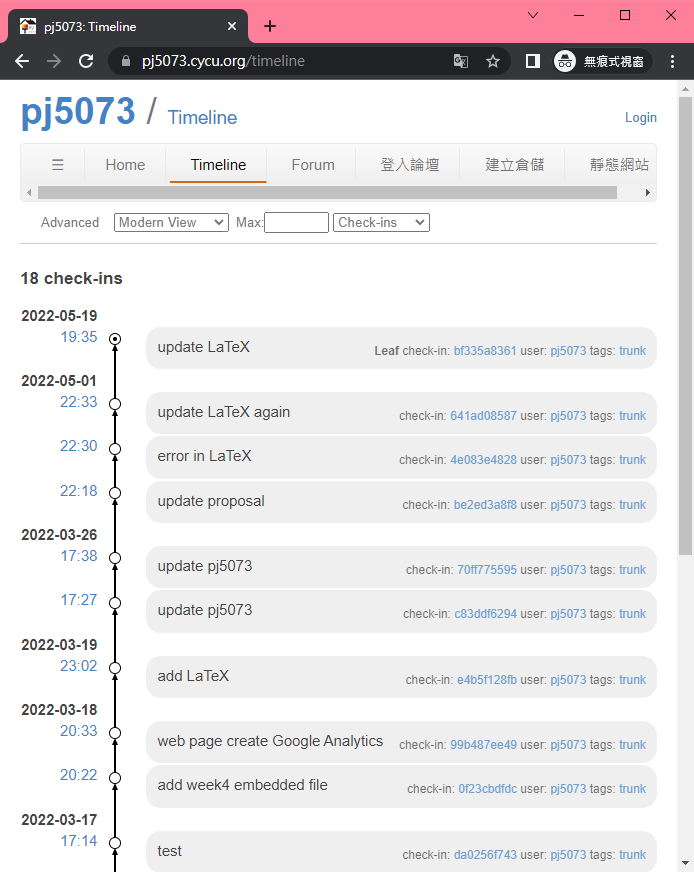
\includegraphics[width=5in]{26}
\caption{\large 本版控制}\label{fig.本版控制}
\end{center}
\end{figure}
\par
\twelve 可以藉由@gm帳號登入,創建屬於個人的倉儲系統,可以藉由版本控制的功能,紀錄確切的時間及完整證明相關資訊,而做為更有信服力的作證資料,創建個人倉儲步驟如(圖.\ref{fig.步驟1-建立倉儲})、(圖.\ref{fig.步驟2-點擊連結})(圖.\ref{fig.步驟3-登入@gm帳號})、(圖.\ref{fig.步驟4-前往連結})、(圖.\ref{fig.步驟5-設定密碼})、(圖.\ref{fig.步驟6-完成})。
\\
\par
\begin{figure}[hbt!]
\begin{center}
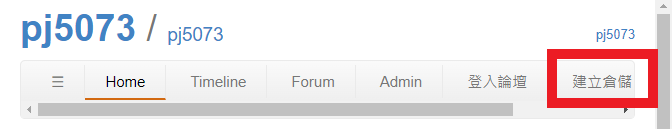
\includegraphics[width=5in]{27}
\caption{\large 步驟1-建立倉儲}\label{fig.步驟1-建立倉儲}
\end{center}
\end{figure}
\par
\begin{figure}[hbt!]
\begin{center}
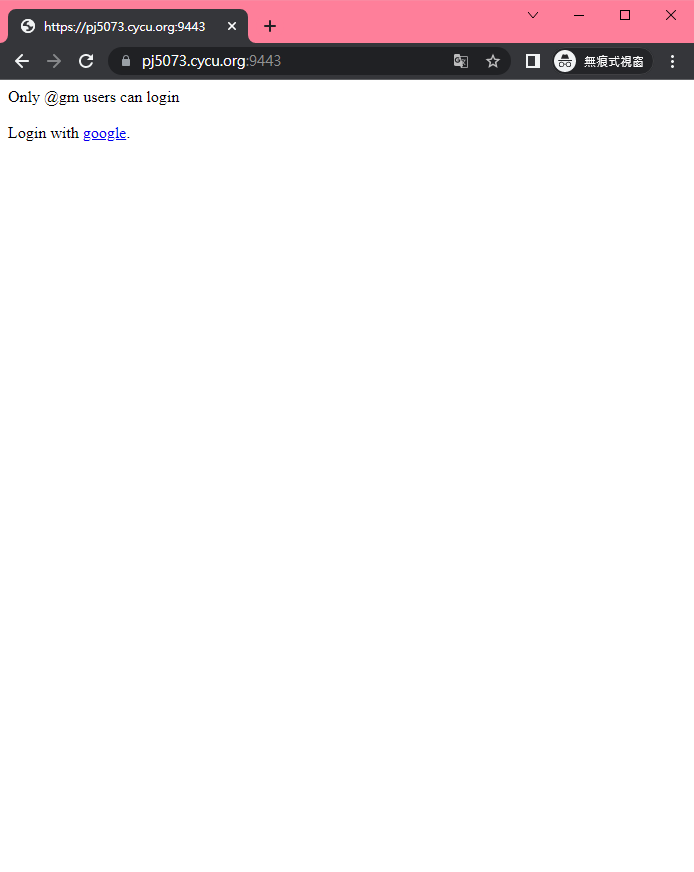
\includegraphics[width=5in]{28}
\caption{\large 步驟2-前往連結}\label{fig.步驟2-點擊連結}
\end{center}
\end{figure}
\par
\begin{figure}[hbt!]
\begin{center}
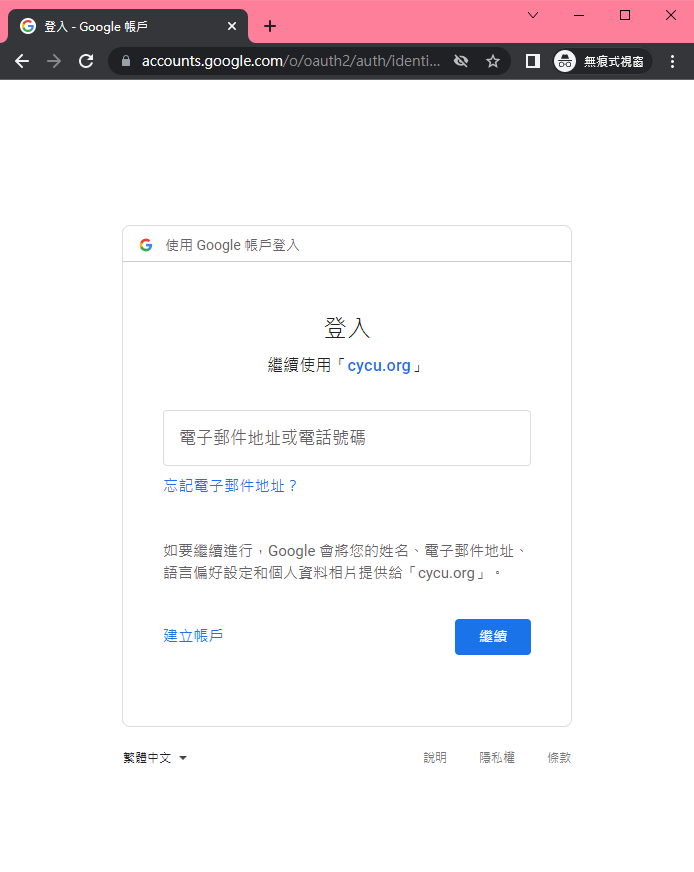
\includegraphics[width=5in]{32}
\caption{\large 步驟3-登入@gm帳號}\label{fig.步驟3-登入@gm帳號}
\end{center}
\end{figure}
\par
\begin{figure}[hbt!]
\begin{center}
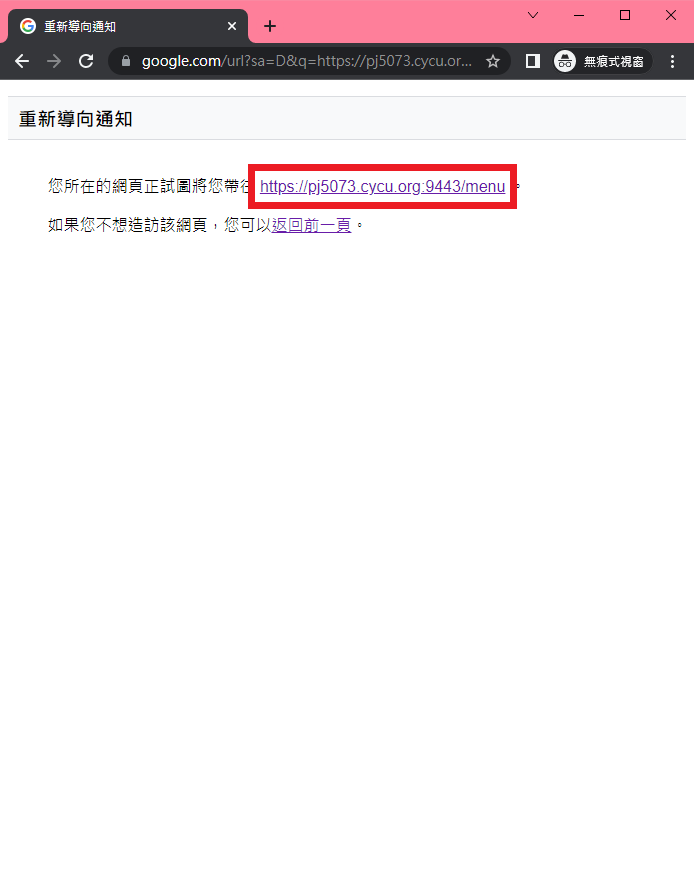
\includegraphics[width=5in]{29}
\caption{\large 步驟4-前往連結}\label{fig.步驟4-前往連結}
\end{center}
\end{figure}
\par
\begin{figure}[hbt!]
\begin{center}
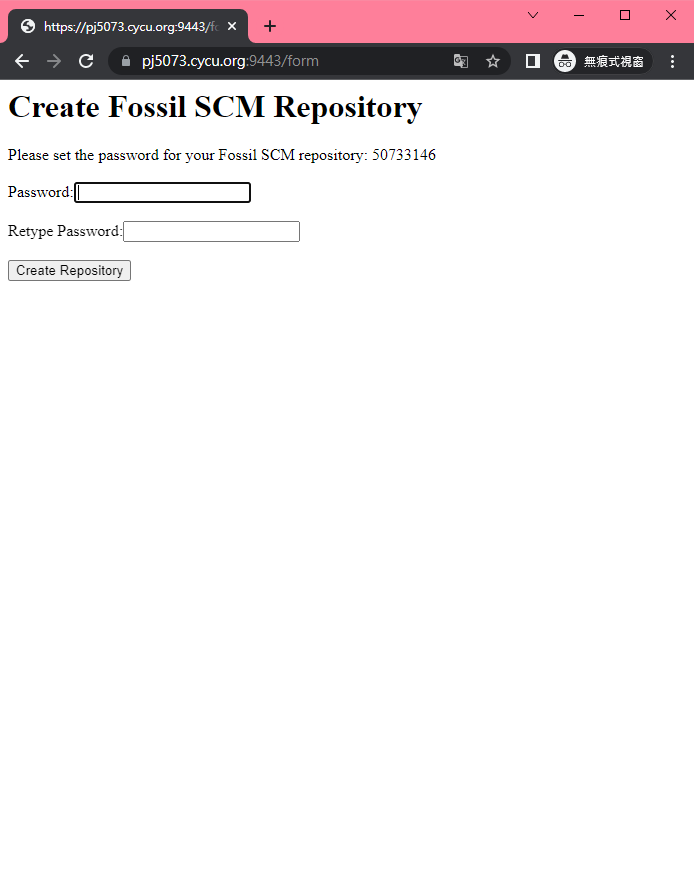
\includegraphics[width=5in]{30}
\caption{\large 步驟5-設定密碼}\label{fig.步驟5-設定密碼}
\end{center}
\end{figure}
\par
\begin{figure}[hbt!]
\begin{center}
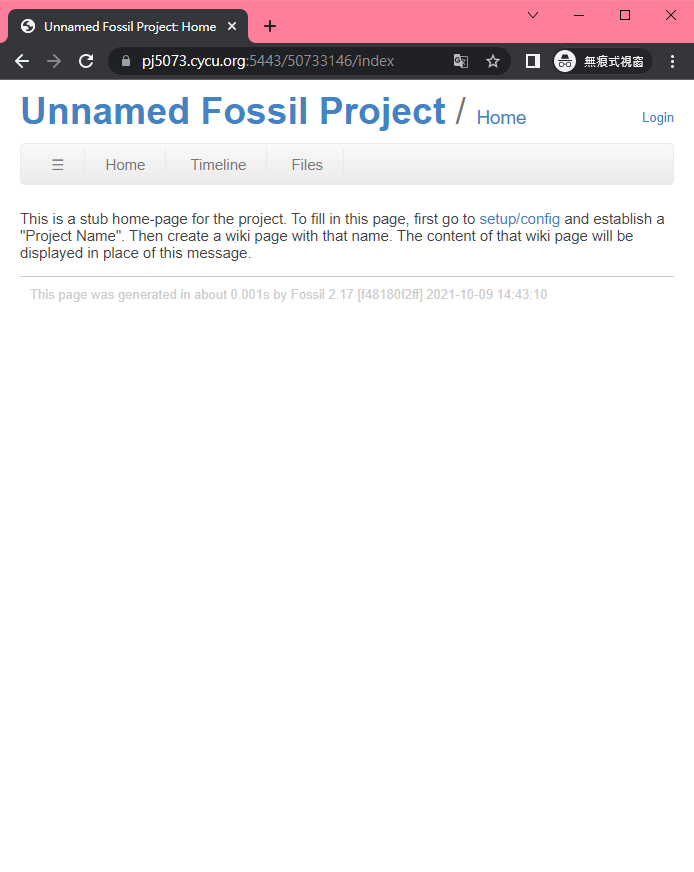
\includegraphics[width=5in]{31}
\caption{\large 步驟6-完成(網址於網域5443/"學號")}\label{fig.步驟6-完成}
\end{center}
\end{figure}
\par


